\iffalse
\documentclass[journal,12pt,twocolumn]{IEEEtran}
%
\usepackage{setspace}
\usepackage{gensymb}
%\doublespacing
\singlespacing

%\usepackage{graphicx}
%\usepackage{amssymb}
%\usepackage{relsize}
\usepackage[cmex10]{amsmath}
%\usepackage{amsthm}
%\interdisplaylinepenalty=2500
%\savesymbol{iint}
%\usepackage{txfonts}
%\restoresymbol{TXF}{iint}
%\usepackage{wasysym}
\usepackage{amsthm}
%\usepackage{iithtlc}
\usepackage{mathrsfs}
\usepackage{txfonts}
\usepackage{stfloats}
\usepackage{bm}
\usepackage{cite}
\usepackage{cases}
\usepackage{subfig}
%\usepackage{xtab}
\usepackage{longtable}
\usepackage{multirow}
%\usepackage{algorithm}
%\usepackage{algpseudocode}
\usepackage{enumitem}
\usepackage{mathtools}
\usepackage{steinmetz}
\usepackage{tikz}
\usepackage{circuitikz}
\usepackage{verbatim}
\usepackage{tfrupee}
\usepackage[breaklinks=true]{hyperref}
%\usepackage{stmaryrd}
\usepackage{tkz-euclide} % loads  TikZ and tkz-base
%\usetkzobj{all}
\usetikzlibrary{calc,math}
\usepackage{listings}
    \usepackage{color}                                            %%
    \usepackage{array}                                            %%
    \usepackage{longtable}                                        %%
    \usepackage{calc}                                             %%
    \usepackage{multirow}                                         %%
    \usepackage{hhline}                                           %%
    \usepackage{ifthen}                                           %%
  %optionally (for landscape tables embedded in another document): %%
    \usepackage{lscape}     
\usepackage{multicol}
\usepackage{chngcntr}
%\usepackage{enumerate}

%\usepackage{wasysym}
%\newcounter{MYtempeqncnt}
\DeclareMathOperator*{\Res}{Res}
%\renewcommand{\baselinestretch}{2}
\renewcommand\thesection{\arabic{section}}
\renewcommand\thesubsection{\thesection.\arabic{subsection}}
\renewcommand\thesubsubsection{\thesubsection.\arabic{subsubsection}}

\renewcommand\thesectiondis{\arabic{section}}
\renewcommand\thesubsectiondis{\thesectiondis.\arabic{subsection}}
\renewcommand\thesubsubsectiondis{\thesubsectiondis.\arabic{subsubsection}}

% correct bad hyphenation here
\hyphenation{op-tical net-works semi-conduc-tor}
\def\inputGnumericTable{}                                 %%

\lstset{
%language=C,
frame=single, 
breaklines=true,
columns=fullflexible
}
%\lstset{
%language=tex,
%frame=single, 
%breaklines=true
%}

\begin{document}
%


\newtheorem{theorem}{Theorem}[section]
\newtheorem{problem}{Problem}
\newtheorem{proposition}{Proposition}[section]
\newtheorem{lemma}{Lemma}[section]
\newtheorem{corollary}[theorem]{Corollary}
\newtheorem{example}{Example}[section]
\newtheorem{definition}[problem]{Definition}
%\newtheorem{thm}{Theorem}[section] 
%\newtheorem{defn}[thm]{Definition}
%\newtheorem{algorithm}{Algorithm}[section]
%\newtheorem{cor}{Corollary}
\newcommand{\BEQA}{\begin{eqnarray}}
\newcommand{\EEQA}{\end{eqnarray}}
\newcommand{\define}{\stackrel{\triangle}{=}}

\bibliographystyle{IEEEtran}
%\bibliographystyle{ieeetr}


\providecommand{\mbf}{\mathbf}
\providecommand{\pr}[1]{\ensuremath{\Pr\left(#1\right)}}
\providecommand{\qfunc}[1]{\ensuremath{Q\left(#1\right)}}
\providecommand{\sbrak}[1]{\ensuremath{{}\left[#1\right]}}
\providecommand{\lsbrak}[1]{\ensuremath{{}\left[#1\right.}}
\providecommand{\rsbrak}[1]{\ensuremath{{}\left.#1\right]}}
\providecommand{\brak}[1]{\ensuremath{\left(#1\right)}}
\providecommand{\lbrak}[1]{\ensuremath{\left(#1\right.}}
\providecommand{\rbrak}[1]{\ensuremath{\left.#1\right)}}
\providecommand{\cbrak}[1]{\ensuremath{\left\{#1\right\}}}
\providecommand{\lcbrak}[1]{\ensuremath{\left\{#1\right.}}
\providecommand{\rcbrak}[1]{\ensuremath{\left.#1\right\}}}
\theoremstyle{remark}
\newtheorem{rem}{Remark}
\newcommand{\sgn}{\mathop{\mathrm{sgn}}}
\providecommand{\abs}[1]{\left\vert#1\right\vert}
\providecommand{\res}[1]{\Res\displaylimits_{#1}} 
\providecommand{\norm}[1]{\left\lVert#1\right\rVert}
%\providecommand{\norm}[1]{\lVert#1\rVert}
\providecommand{\mtx}[1]{\mathbf{#1}}
\providecommand{\mean}[1]{E\left[ #1 \right]}
\providecommand{\fourier}{\overset{\mathcal{F}}{ \rightleftharpoons}}
%\providecommand{\hilbert}{\overset{\mathcal{H}}{ \rightleftharpoons}}
\providecommand{\system}{\overset{\mathcal{H}}{ \longleftrightarrow}}
	%\newcommand{\solution}[2]{\textbf{Solution:}{#1}}
\newcommand{\solution}{\noindent \textbf{Solution: }}
\newcommand{\cosec}{\,\text{cosec}\,}
\providecommand{\dec}[2]{\ensuremath{\overset{#1}{\underset{#2}{\gtrless}}}}
\newcommand{\myvec}[1]{\ensuremath{\begin{pmatrix}#1\end{pmatrix}}}
\newcommand{\mydet}[1]{\ensuremath{\begin{vmatrix}#1\end{vmatrix}}}
%\numberwithin{equation}{section}
\numberwithin{equation}{subsection}
%\numberwithin{problem}{section}
%\numberwithin{definition}{section}
\makeatletter
\@addtoreset{figure}{problem}
\makeatother

\let\StandardTheFigure\thefigure
\let\vec\mathbf
%\renewcommand{\thefigure}{\theproblem.\arabic{figure}}
\renewcommand{\thefigure}{\theproblem}
%\setlist[enumerate,1]{before=\renewcommand\theequation{\theenumi.\arabic{equation}}
%\counterwithin{equation}{enumi}


%\renewcommand{\theequation}{\arabic{subsection}.\arabic{equation}}

\def\putbox#1#2#3{\makebox[0in][l]{\makebox[#1][l]{}\raisebox{\baselineskip}[0in][0in]{\raisebox{#2}[0in][0in]{#3}}}}
     \def\rightbox#1{\makebox[0in][r]{#1}}
     \def\centbox#1{\makebox[0in]{#1}}
     \def\topbox#1{\raisebox{-\baselineskip}[0in][0in]{#1}}
     \def\midbox#1{\raisebox{-0.5\baselineskip}[0in][0in]{#1}}

\vspace{3cm}


\title{Problem: 9.10.6.8}
\author{Nikam Pratik Balasaheb (EE21BTECH11037)}





% make the title area
\maketitle

\newpage

%\tableofcontents

\bigskip

\renewcommand{\thefigure}{\theenumi}
\renewcommand{\thetable}{\theenumi}
%\renewcommand{\theequation}{\theenumi}

\section{Problem}

\section{Solution}
\fi

\begin{enumerate}

\item Let the vertices of the triangle ABC be:
	\begin{align}
		\vec{B} &= \myvec{0\\0}\\
		\vec{C} &= \myvec{a\\0}\\
		\vec{A} &= c\myvec{\cos{\theta}\\ \sin{\theta}}
	\end{align}
	For ease of calculation let's assume $\theta = 60{\degree}, a = c = 5$.

\item side length $b$ is given by:
	\begin{align}
		b &= \norm{A-C}\\
		&= \norm{ \myvec{ c\cos{\theta} - a \\ c\sin{\theta}}} \\
		&= \sqrt{a^2 + c^2 - 2ac \cos{\theta}}\\
	\end{align}

\item Circumcenter of triangle ABC:\\
	Circumcenter of triangle can be found by calculating point of intersection of perpedicular bisectors of two sides.
	\begin{enumerate}
	\item perpendicular bisector of side BC:
		\begin{align}
			\brak{\vec{C}-\vec{B}}^{\top}\brak{\vec{x}- \frac{\vec{C}+\vec{B}}{2}} &= 0\\
			\brak{\vec{C}-\vec{B}}^{\top} \vec{x} &= \frac{\norm{\vec{C}}^2 -\norm{\vec{B}}^2}{2}\\
			\vec{C}^{\top}\vec{x} &= \frac{a^2}{2} 
		\end{align}
	\item perpendicular bisector of side AB:
		\begin{align}
			\vec{A}^{\top}\vec{x} &= \frac{c^2}{2}
		\end{align}
	\end{enumerate}
	
	Therefore, the circumcenter is given by:
		\begin{align}
			\myvec{ a & 0\\ c \cos{\theta} & c \sin{\theta}} \vec{O} &= \myvec{ \frac{a^2}{2} \\ \frac{c^2}{2}}
		\end{align}

\item Circumradius of triangle ABC,
	\begin{align}
		R &= \norm{\vec{A}-\vec{O}}
	\end{align}
\item For Circumcircle of triangle ABC,
	Writing equation of circle in form $\vec{x}\vec{V}\vec{x}^{\top} 
		\vec{u}^{\top}\vec{x} + f = 0$,
		\begin{align}
			\vec{V} &= \myvec{1&0\\0&1}\\
			\vec{u} &= -\vec{O}\\
			f &= \norm{\vec{O}}^2 - R^2\\
			&= 2\vec{O}^{\top}\vec{A} - \norm{\vec{A}}^2
		\end{align}

\item angular bisectors:
	Expressing the line equations in form $\vec{x} = \vec{h} + \mu\vec{m}$,
	\begin{enumerate}
		\item Angular Bisector of angle A:
			\begin{align}
				\vec{m} &= \brak{\vec{C} -\vec{A}} + \brak{ \vec{B} -\vec{A}}\\
					&= \vec{B} + \vec{C} -2\vec{A}\\
				\vec{h} &= \vec{A}
			\end{align}
		\item Angular Bisector of angle B:
			\begin{align}
				\vec{m} &= \brak{\vec{C} -\vec{B}}+ \brak{ \vec{A} -\vec{B}}\\
				        &= \vec{A} + \vec{C} -2\vec{B}\\
				\vec{h} &= \vec{A}
			\end{align}
		\item Angular Bisector of angle C:
			\begin{align}
				\vec{m} &= \brak{\vec{A} -\vec{C}}+ \brak{ \vec{B} -\vec{C}}\\
			                &= \vec{A} + \vec{B} -2\vec{C}\\
			\vec{h} &= \vec{C}
			\end{align}
	\end{enumerate}


\item The point of intersection of any line $\vec{x}= \vec{h} + \mu\vec{m}$ and conic $\vec{x}^{\top}\vec{V}\vec{x} +2\vec{u}^{\top}\vec{x} +f =0$:

	\begin{multline}
        \mu_i = \frac{1}{\vec{m}^{\top}\vec{V}\vec{m}} \brak{-m^{\top}\brak{\vec{V}\vec{h}+\vec{u}} \pm \sqrt{\brak{\vec{m}^{\top}\brak{\vec{V}\vec{h}+\vec{u}}}^2 - \text{g}\brak{\vec{h}}\brak{\vec{m}^{\top}\vec{V}\vec{m}}}}
\end{multline}

where,
\begin{align}
        \text{g}\brak{\vec{h}} = \vec{h}^{\top}\vec{V}\vec{h} + 2\vec{u}^{\top}\vec{h} +f
\end{align}

\item The points of intersection D, E and F are found using above method. Refer \texttt{codes/9.10.6.8.py}. The resulting $ \vec{D} , \vec{E}, \vec{F}$ are given in table \ref{tab:chapters/9/10/6/8/POIs}. 
\begin{table}[h!]
\centering
	\input{chapters/9/10/6/8/tables/DE&F.tex}
        \caption{Table}		\label{tab:chapters/9/10/6/8/POIs}
\end{table}


\item The desired angle i.e $\angle DEF$ is found by using,
	\begin{align}
		\cos\brak{\angle DEF} &= \frac{ \brak{\vec{D}-\vec{E}}^{\top} \brak{ \vec{F}-\vec{E}} } { \norm{\vec{D}-\vec{E}} \norm{\vec{F}-\vec{E}} }
	\end{align}

\item In \texttt{codes/9.10.6.8.py}, the problem is solved for $a =c = 5$ and $ \theta = 60 \degree$.\\
	It is seen that the angle $\angle DEF$ is $ 60 \degree$ which satsifies the statement to be proved.
\end{enumerate}

\begin{table}[h!]
\centering
        %%%%%%%%%%%%%%%%%%%%%%%%%%%%%%%%%%%%%%%%%%%%%%%%%%%%%%%%%%%%%%%%%%%%%%
%%                                                                  %%
%%  This is a LaTeX2e table fragment exported from Gnumeric.        %%
%%                                                                  %%
%%%%%%%%%%%%%%%%%%%%%%%%%%%%%%%%%%%%%%%%%%%%%%%%%%%%%%%%%%%%%%%%%%%%%%

\begin{tabular}[]{|c|c|c|}
\hline
Parameter	& Value	& Desription \\ \hline
$a$	& 5 & length of side opposite to Vertex $\vec{A}$\\ \hline
	$c$	& 5 & length of side opposite to vertex $\vec{C}$\\ \hline
	$\theta$		& $60\degree$ & $\angle{ABC}$\\ \hline
\end{tabular}

        \caption{Table}
        \label{tab:chapters/9/10/6/8/}
\end{table}

\begin{figure}[h]
  \centering
   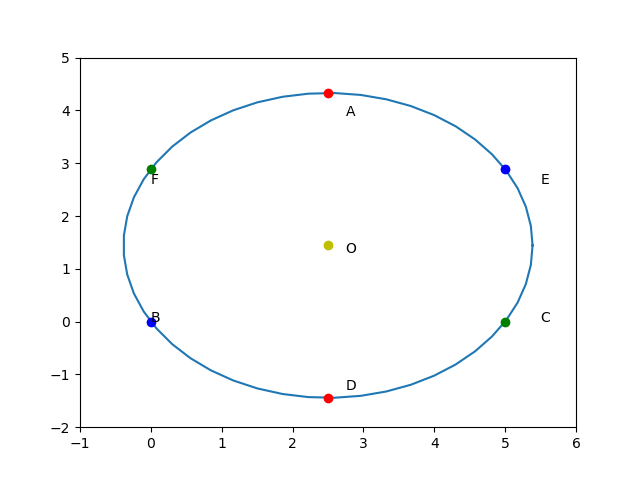
\includegraphics[width=\linewidth,height = \linewidth]{chapters/9/10/6/8/figs/Figure_1.png}
   \caption{Figure}
   \label{fig:chapters/9/10/6/8/}
\end{figure}




